\subsection{Bearing Off}\label{sec:bearing-off}
To bear off, a player must first make a \textit{Set} by stacking two of their own cubes of like value, similar to Pinching.

Sets are special because they break the normal movement rules:
\begin{enumerate}
    \item Sets do not rotate before moving. If the cubes show 16, then they'll show 16 even after moving.
    \item Sets can jump over \textbf{any number} of adjacent other cubes or sets as part of their movement (see Figure~\ref{fig:jump}). This jump counts as just one move. Single cubes \textbf{cannot} jump.
    \item When moving sets players can \textit{add together} the results of both dice. This is not possible when moving cubes.
    \item Sets cannot pinch, only jump.
    \item Sets must move directly towards the pin on the board, and are not allowed to meander.
\end{enumerate}
\begin{figure}[!h]
    \centering
    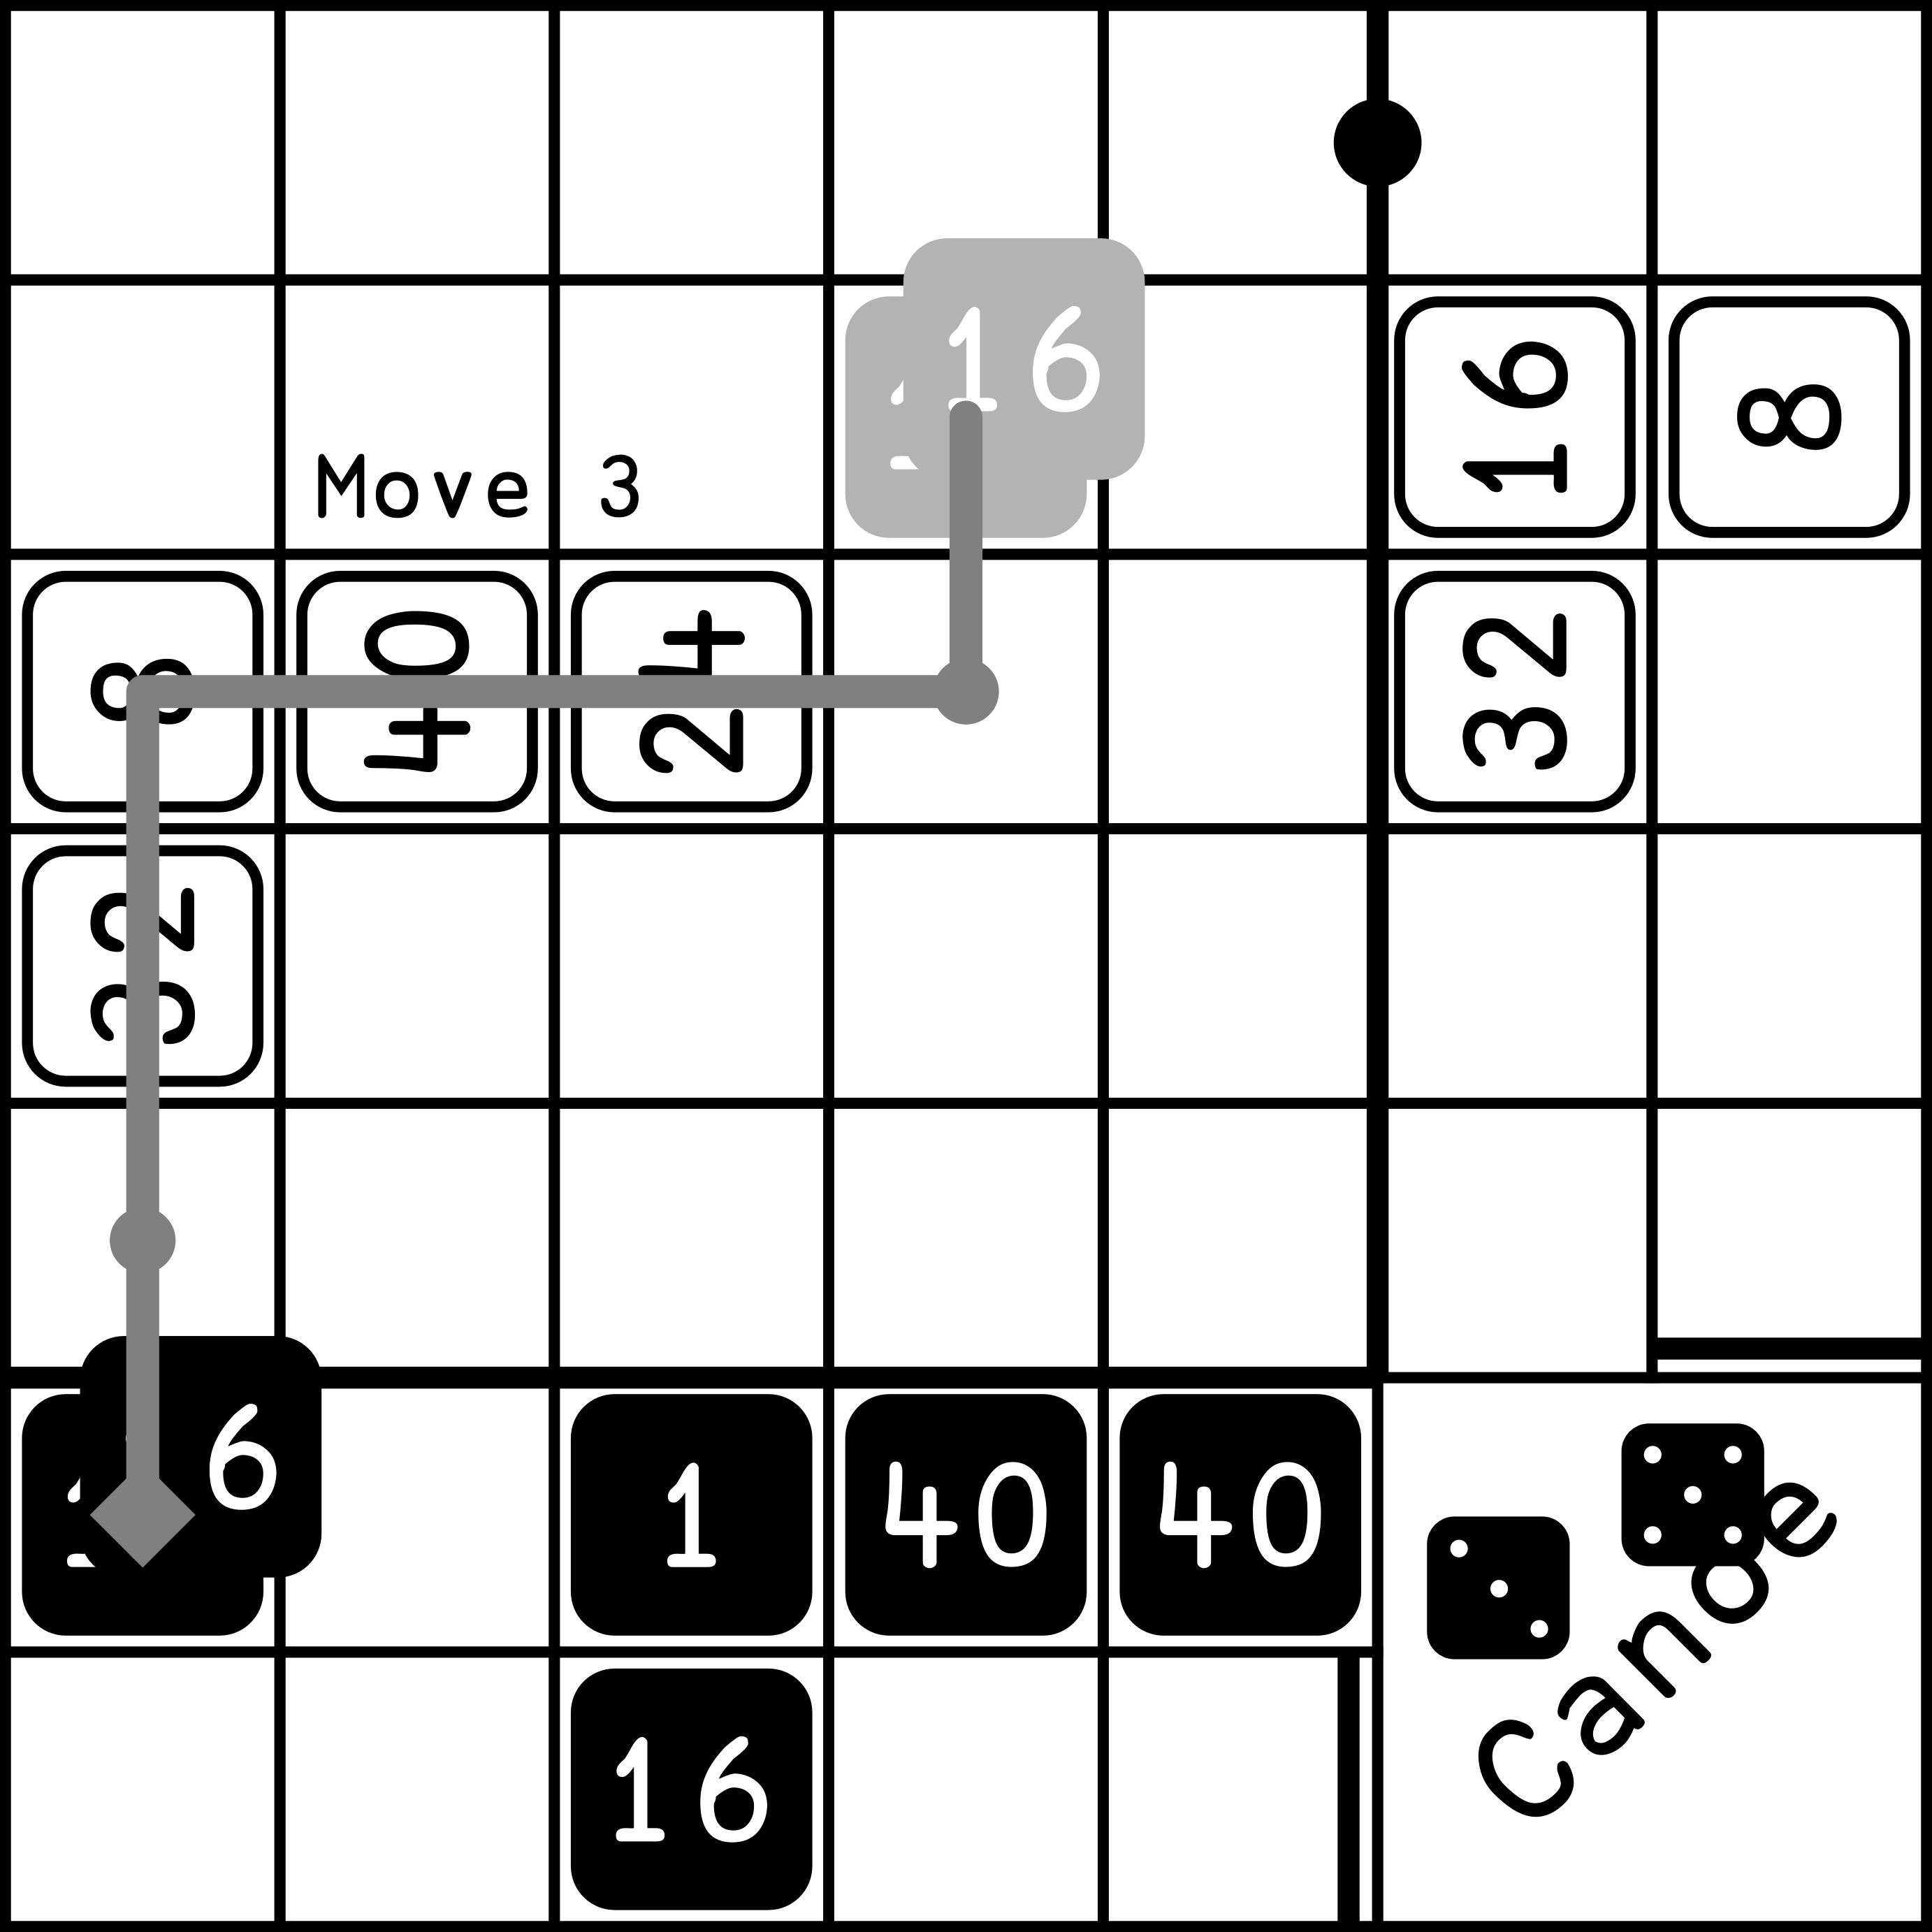
\includegraphics[width=8cm]{../graphics/jump}
    \caption{Example Jump}
    \label{fig:jump}
\end{figure}
To then bear off, a player must move the stack of cubes over the pin (black dot) on the starting line and into the bank, before then having to move towards the leather patch and over the line on the backmost row.

\paragraph{Jumping Example}
Figure~\ref{fig:jump} illustrates an example jump.
Black rolled a \epsdice{3} and a \epsdice{5}, and wishes to move their stack of 16s.
To get into the bank as quickly as possible, Black uses their \epsdice{3} and makes use of stacks' ability to jump over other pieces by first moving one down, then all the way over all of Ivory's pieces as the second move, only to end up inside the bank with a third move.

\paragraph{Note} Sets cannot be formed with cubes that have just left the bank.

\paragraph{Note} To bear off, a player needs the exact number or number combination to make it to the leather patch. If the roll is not an exact match, it will not work.

\subsubsection{Canoe}
The first time a player bears off their cubes, \textit{both} of the cubes are pocketed for scoring.

All subsequent times, only one cube is pocketed, while the other is discarded, never to be seen again.

\subsubsection{Seventh Cube}
Once all but the last cube have been pinched or borne off, the seventh cube can then be borne off all by itself.
Doing so successfully sweeps the opponent's remaining cubes into the pocket as points.

Like a set, the seventh cube can also combine the results of the two dice for better reach.
Also like a set, the seventh cube must bear off as soon as possible.